% !TeX program = xelatex
\documentclass[10.5pt,a4paper,fontset=fandol]{ctexart}
\usepackage[a4paper,top=1.35cm,bottom=1.25cm,left=1.50cm,right=1.50cm]{geometry}
\usepackage{graphicx,tabularx,array,enumitem,hyperref,xcolor,fancyhdr,needspace}
\usepackage{fontspec}

\setmainfont{TeX Gyre Termes}
\setCJKmainfont{FandolSong-Regular}[BoldFont=FandolSong-Bold]
\hypersetup{colorlinks=true,urlcolor=black,pdfauthor={郑新楠},pdftitle={郑新楠简历}}
\pagestyle{fancy}\fancyhf{}\renewcommand{\headrulewidth}{0pt}
\fancyfoot[C]{\small\thepage}
\setlength{\parindent}{0pt}
\setlength{\parskip}{0pt}
\linespread{1.18}
\setlist{nosep,leftmargin=1.55em,labelsep=.45em}

\newcommand{\ressection}[1]{%
  \needspace{3\baselineskip}\vspace{.55em}%
  {\zihao{4}\bfseries #1}\par\vspace{-.45em}%
  \noindent\rule{\textwidth}{0.45pt}\vspace{.30em}}
\newcommand{\entry}[4]{%
  \begin{tabularx}{\textwidth}{@{}>{\raggedright\arraybackslash}X>{\raggedleft\arraybackslash}p{3.8cm}@{}}
    \textbf{#1} & {\color{gray}#2}\\[-.08em]
    #3 & {\color{gray}#4}
  \end{tabularx}\vspace{.18em}}
\newcommand{\dateditem}[3]{%
  \begin{tabularx}{\textwidth}{@{}>{\raggedright\arraybackslash}X>{\raggedleft\arraybackslash}p{2.1cm}@{}}
    \textbf{#1} & {\color{gray}#2}\\[-.1em]
    #3 &
  \end{tabularx}\vspace{.18em}}
\newcommand{\project}[4]{%
  \begin{tabularx}{\textwidth}{@{}>{\raggedright\arraybackslash}X>{\raggedleft\arraybackslash}p{2.7cm}@{}}
    \textbf{#1} & {\color{gray}#2}\\[-.1em]
    #3 &
  \end{tabularx}
  \begin{itemize}[leftmargin=1.45em,topsep=.05em,itemsep=.05em]
    #4
  \end{itemize}\vspace{.12em}}

\begin{document}
\thispagestyle{fancy}

\begin{center}
  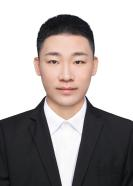
\includegraphics[width=2.65cm,height=3.45cm,keepaspectratio]{portrait.jpg}\\[-.1em]
  {\zihao{2}\bfseries 郑新楠，博士}\\[.45em]
  邮箱：\href{mailto:xinnan.zheng@ieee.org}{xinnan.zheng@ieee.org}\quad|\quad
  电话：+86 13663501199\quad|\quad 微信：MasterZXN\quad|\quad 出生年月：2000 年 1 月\\[-.05em]
  \href{https://scholar.google.com/}{Google 学术主页}
\end{center}

\ressection{个人优势}
\textbf{政治背景：}中共党员（2022 年 5 月加入）。具备坚定的政治立场和良好的组织纪律性，责任心强，能够在团队中发挥模范带头作用。\par\vspace{.38em}
\textbf{教育背景：}曼彻斯特大学电气与电子工程博士，研究方向覆盖电磁无损检测与电磁仿真技术（NDT、脉冲/多频涡流 ECT/PECT、电容/电磁层析 ECT/EMT）、传感器硬件与算法设计、深度学习与软硬件协同设计；本科为北京工业大学 \& 都柏林大学学院国际联培双学位，综测 GPA 4.05/4.2，电子信息工程专业第 1 毕业。\par\vspace{.38em}
\textbf{学术成果：}个人学术总引用量达 170 次，围绕脉冲/多频涡流检测与电磁层析发表 20 余篇 SCI/EI 论文，其中 25 篇发表于 JCR 一区/Top 期刊；第一/共同作者代表作包括 \textit{IEEE Transactions on Instrumentation and Measurement}、\textit{IEEE Transactions on Magnetics}、\textit{NDT \& E International}、\textit{Measurement} 等，工作涵盖 AI 协同测量、传感器设计、材料表征分析与 AR 可视化智能测量等方向。\par\vspace{.38em}
\textbf{项目经验：}具备从传感器与线圈设计、数据采集与信号调理、嵌入式/上位机软件，到学习算法建模与工程化验证的全流程落地能力；主导/参与多频与脉冲涡流检测仪器与传感器开发、电磁/电容层析传感器等原型研发，并在基于脉冲涡流检测系统的真实金属板件厚度与缺陷检测任务中完成性能对标与工程应用验证，该成果进入商业化准备阶段。并有多次投资项目路演以及创新创业大赛的负责人与答辩人经历。\par\vspace{.38em}
\textbf{荣誉奖励：}国家优秀自费留学生奖学金、中英青年创新大赛英国区域赛国际二等奖、国家奖学金、北京市三好学生、都柏林大学学院杰出学子、小米特等奖学金等个人荣誉 17 项；累计获得国家级/省部级等各类学科竞赛奖项 23 项。

\ressection{教育背景}
\entry{曼彻斯特大学（The University of Manchester）}{2022.09 -- 2026.06（预计）}{博士研究生—电气与电子工程\newline 研究方向：电磁仿真、多频/脉冲涡流无损探伤、传感器设计、AI 协同测量、AR 可视化测量。}{英国 · 曼彻斯特}
\entry{都柏林大学（University College Dublin）}{2018.09 -- 2022.06}{本科—电子信息工程\quad|\quad GPA 3.84/4.2，专业第 4/59\newline 核心课程：微控制器、嵌入式、数字信号处理、电路与系统、信号与系统、控制理论、通信等。}{爱尔兰 · 都柏林}
\entry{北京工业大学}{2018.09 -- 2022.06}{本科—电气工程及其自动化\quad|\quad GPA 3.84/4.2，专业第 4/59\newline 核心课程：高等数学、线性代数、C 语言、Python、电路分析、电磁场、Java、复变函数等。}{中国 · 北京}

\ressection{项目经历}
\project{金属厚度检测脉冲涡流仪器开发}{2022.09 -- 至今}{项目职责：仪器主板 PCB 线路设计，前端 UI 界面优化，传感器设计，仪器处理算法设计。}{
  \item 开发金属厚度检测 PEC 仪器，达到行业领先准确率，现进入商业化阶段（B2B）。
  \item 设计嵌入式金属厚度识别算法，能够在复杂工业变化环境中保持高测量准确率，达行业领先水平。
  \item 设计成套小型便携式传感器，达到行业同量级传感器最佳准确率与性能，进入商业化阶段（B2B）。}
\project{房屋建筑结构实时 AR 成像检测系统}{2024.06 -- 至今}{项目职责：系统算法设计与实现}{
  \item 基于金属厚度检测仪、iTransformer 深度学习算法与 Unity AR 系统研发出房屋钢筋结构三维实时成像系统，延时低于 20 ms，误差率不超过 1\%。}
\project{实时血液成分分析电磁层析成像系统}{2025.02 -- 至今}{项目职责：传感器与算法设计}{
  \item 通过设计小型高灵敏 EMT 传感器检测血液中含量为 mM 级别的成分，从而达到疾病分析与预测的效果。所设计出的探头灵敏度处于行业顶尖水平。}

\ressection{荣誉与奖项}
\dateditem{中英青年创新大赛英国区域赛——国际二等奖}{2025}{团队项目获评国际二等奖（创新/落地性）。}
\dateditem{国家优秀自费留学生奖学金}{2024}{国家留学基金委面向在外优秀自费留学生的高层次奖学金（每年全球仅有 650 个名额）。}
\dateditem{国家奖学金}{2021}{教育部国家级最高荣誉奖学金（前 0.1\%）。}
\dateditem{北京市三好学生}{2021}{综合成绩与表现卓越（前 0.1\%）。}
\dateditem{都柏林大学学院杰出学子（UCD Outstanding Student）}{2020}{校级综合表现优秀（前 0.6\%）。}
\dateditem{北京工业大学小米特等奖学金}{2020}{校企联合高额奖学金（前 0.1\%）。}

\ressection{相关经验}
\dateditem{曼彻斯特大学研究生助教}{2022.09 -- 至今}{课程：电子电路设计 II、传感器信号处理与成像、机器人系统等\newline 职责：课堂与实验指导、作业/项目答疑、实验落地支持等。}
\dateditem{都柏林大学学院助教}{2021 -- 2022}{课程：电路与系统、信号与系统、电子电路与理论\newline 职责：课堂协助、实验指导、作业批改与答疑，支持课程教学组织与学生辅导。}
\dateditem{学习委员}{2018.09 -- 2022.06}{职责：负责班级学习事务协调、组织学业交流与资料整理，协助教师与辅导员开展学风建设。}
\dateditem{院团委科协部门成员}{2018.09 -- 2019.06}{职责：参与院级科技创新活动策划与执行，协助组织讲座与竞赛。负责活动宣传与资料整理，增强团队协作与执行能力，工作表现获师生认可。}

\ressection{技能}
\textbf{编程：}Python，C/C++，Java，MATLAB，LaTeX\quad|\quad\textbf{嵌入式：}STM32（外设驱动/接口通信、上位机联调）\par\vspace{.35em}
\textbf{数据库：}MySQL，PostgreSQL\quad|\quad\textbf{网页开发：}HTML，CSS，JavaScript\par\vspace{.35em}
\textbf{研究与工程：}无损检测（NDT），多频/脉冲涡流检测（MFEC/PECT），电容/电磁层析成像（ECT/EMT），信号处理，深度学习/机器学习，软硬件协同设计，传感器/线圈设计与上位机开发

\ressection{学术论文发表}
\begin{enumerate}[leftmargin=1.65em,itemsep=.12em,parsep=0pt]
\item Diffusion Velocity of Eddy Current in Metallic Plates Using Point-Tracing Method \textbf{第一作者}，JCR SCI 一区，2024，\textit{IEEE Transactions on Magnetics}，链接
\item Analyzing the Permeability Distribution of Multilayered Specimens Using Pulsed Eddy-Current Testing with Multi-Scale 1D-ResNet \textbf{第一作者}，JCR SCI 一区，2024，\textit{NDT \& E International} 149:103247，链接
\item High-Efficiency Method for Diffusion Velocity of Eddy Current in Metallic Plates \textbf{第一作者}，JCR SCI 一区，2025，\textit{Measurement} 250:117046，链接
\item Exploring the Effect of Probe Size and Lift-Off on Footprint in Pulsed Eddy Current Testing \textbf{第一作者}，JCR SCI 一区，2025，\textit{Proc. IEEE I2MTC}，链接
\item Measurement of Finite Plate Size in Pulsed Eddy Current Testing \textbf{通讯作者}，JCR SCI 一区，2025，\textit{Measurement} 251:117202，链接
\item Thickness Measurement and Surface-Defect Detection for Metal Plate Using Pulsed Eddy Current Testing and Optimized Res2Net Network \textbf{第二作者}，JCR SCI 一区，2024，\textit{IEEE Transactions on Instrumentation and Measurement}，链接
\item Simultaneous Carbon Fiber Layer Thickness and Direction Measurement and Identification Using a Novel Eddy Current Sensor and Simplified Multi-Scale 1D-ResNet Network \textbf{第二作者}，JCR SCI 一区，Jan 2025，\textit{Measurement}，链接
\item An Innovative Eddy-Current Sensor with E-Core Ferrite Resistant to Lift-Off and Tilt Effects \textbf{第二作者}，JCR SCI 一区，2024，\textit{Nondestructive Testing and Evaluation}，链接
\item Inspection of Defects Depth for Stainless-Steel Sheets Using 4-Coil Excitation Sensor and Deep Learning \textbf{第二作者}，JCR SCI 一区，2023，\textit{IEEE Transactions on Instrumentation and Measurement}，链接
\item Automatic Detection and Imaging of Rivet Hole Defects for Aircraft Structures With Optimized Sensor Array Using Eddy Current Method and Image Analysis \textbf{第二作者}，JCR SCI 一区，2022，\textit{IEEE Sensors Journal}，链接
\item Evaluation of Defects Depth for Metal Sheets Using Four-Coil Excitation Array Eddy Current Sensor and Improved ResNet18 Network \textbf{第二作者}，JCR SCI 一区，2024，\textit{IEEE Sensors Journal}，链接
\item Real-Time Tunnel-Magnetoresistive-Based Pulsed Eddy Current Testing With Deep Learning \textbf{第三作者}，JCR SCI 一区，2024，\textit{IEEE Sensors Journal}，链接
\item Simultaneous Measurements of Metal Plate Thickness and Defect Depth Using Low Frequency Sweeping Eddy Current Testing \textbf{第三作者}，JCR SCI 一区，2024，\textit{Measurement} 233:114687，链接
\item Real-time automatic thickness recognition using pulse eddy current with deep learning \textbf{第三作者}，JCR SCI 一区，2023，\textit{Proc. IEEE I2MTC}，链接
\item Simultaneous measurements of metal thickness and defect depth using low frequency sweeping eddy current testing \textbf{第三作者}，JCR SCI 一区，2024，\textit{Proc. IEEE I2MTC}，链接
\item Measurement of permeability and radius for asymmetric cylinders with double coils using a simplified analytical model of eddy current testing \textbf{第三作者}，JCR SCI 一区，2026，\textit{NDT \& E International}，链接
\item Simultaneous Estimation of Conductivity and Radial Eccentricity of Metallic Cylinders Using Eddy Current Testing \textbf{第三作者}，JCR SCI 一区，2025，\textit{IEEE Transactions on Instrumentation and Measurement}，链接
\item Fast Real-time Electromagnetic Tomography System for Size Prediction and Material and Position Classification \textbf{第三作者}，JCR SCI 一区，2025，\textit{IEEE Transactions on Instrumentation and Measurement}，链接
\item Fast inversion of parameters on Jiles--Atherton hysteresis model based on physics-guided deep learning network \textbf{第四作者}，JCR SCI 一区，2025，\textit{Engineering Applications of Artificial Intelligence}，链接
\item Analytical Modeling of Eddy Current Testing for Asymmetric Cylinders and Estimation of Radii and Electromagnetic Properties \textbf{第四作者}，2025，\textit{IEEE I2MTC}（会议），链接
\item ECTAR: An Integrated Augmented Reality and Eddy Current Array System for Non-destructive Testing of Metallic Plate \textbf{第四作者}，2025，\textit{IEEE I2MTC}（会议），链接
\item Through thickness inspection of layered magnetic material using pulsed eddy-current testing \textbf{第五作者}，JCR SCI 一区，2023，\textit{IEEE Transactions on Instrumentation and Measurement}，链接
\item Sensitivity Focusing Through Coil Angle Variation in Eddy Current Testing \textbf{第五作者}，JCR SCI 一区，2024，\textit{IEEE Transactions on Magnetics}，链接
\item Tilt Effects in Pulsed Eddy Current Measurements \textbf{第五作者}，JCR SCI 一区，2025，\textit{Proc. IEEE I2MTC}，链接
\item Sensitivity map centralisation across different lift-offs through tilted coils \textbf{第六作者}，JCR SCI 一区，2025，\textit{Measurement}，链接
\item A size-distinguishing miniature electromagnetic tomography sensor for small object detection \textbf{第七作者}，JCR SCI 一区，2024，\textit{NDT \& E International}，链接
\end{enumerate}

\end{document}
